\documentclass[12pt]{article}
\usepackage[portuguese]{babel}
\usepackage{amsmath}
\usepackage{graphicx}
\newcommand{\numpy}{{\tt numpy}}   

\topmargin -.5in
\textheight 9in
\oddsidemargin -.25in
\evensidemargin -.25in
\textwidth 7in

\begin{document}
\medskip
\author{Tradução Juan Carlos Teran}
\title{Mecânica Estadística}
\maketitle
O propósito deste capítulo é revisar alguns conceitos fundamentais da termodinâmica, que formam uma base essencial para o estudo da mecânica estatística. Os problemas 2.1-2.3 lidam com a primeira e a segunda leis e os conceitos associados de temperatura e potenciais termodinâmicos. Uma variedade de relações entre grandezas termodinâmicas, incluindo as relações de Maxwell, pode ser derivada desses princípios básicos, juntamente com as regras do cálculo diferencial, e os métodos para obter tais relações são ilustrados nos problemas 2.4 e 2.5. O problema 2.6 ilustra a natureza das mudanças de entropia em processos irreversíveis, enquanto os problemas 2.7-2.9 investigam as equações de estado de sistemas simples e suas consequências para vários processos termodinâmicos. Finalmente, o problema 2.10 lida com o tratamento termodinâmico de um material magnético e o problema 2.11 trata o comportamento de gases relativísticos em um cenário cosmológico.


 \begin{itemize}
     \item \textbf{Problema 2.1} Mostre que a energia livre de Helmholtz $F(T, V)$ de um sistema cujo volume é $V$ em contato com um banho térmico a temperatura $T$ é mínima no equilíbrio. Analogamente, mostre que a energia livre de Gibbs $G(T, P)$ de um sistema em contato com um banho a temperatura $T$ e pressão $P$ é mínima no equilíbrio.

     \textbf{Resposta:}
     Consideremos um sistema cujo volume $V$ é fixo e é colocado em contato com um banho térmico à temperatura $T$. Enquanto o sistema não estiver em equilíbrio com o banho, não podemos atribuir-lhe uma temperatura definida, portanto sua energia livre de Helmholtz $F$ não é uma função bem definida de temperatura e volume. Podemos, no entanto, tentar definir uma energia livre de não-equilíbrio por:
     \begin{equation*}
         F = U - TS
     \end{equation*}
     
     Aqui, entendemos por $U$ a energia interna do sistema, que está bem definida mesmo fora do equilíbrio, e por $T$ a temperatura do banho térmico (que também será a temperatura do sistema uma vez que o equilíbrio seja atingido). A entropia $S$ de não-equilíbrio do sistema não é simplesmente uma função de $U$ e $V$, mas depende dos detalhes do estado de não-equilíbrio. Podemos recorrer à declaração de Clausius da segunda lei para escrever a desigualdade:
     \begin{equation}
         \delta S \geq \frac{\delta Q}{T}
     \end{equation}
     onde $\delta Q$ é uma quantidade de calor transferida do banho térmico para o sistema. Como o volume do sistema é constante, nenhum trabalho é realizado enquanto esse calor é transferido, então a mudança na energia interna do sistema é $\delta U = \delta Q$. Como a temperatura $T$ do banho térmico é fixa, deduzimos que:
     \begin{equation}
         \delta F = \delta U - T \delta S = \delta Q - T \delta S \leq 0.
     \end{equation}
     Assim, $F$ sempre diminui à medida que o sistema se aproxima do equilíbrio e atinge um mínimo quando o equilíbrio é alcançado.
    
     Outra forma de abordar o problema é considerando a variação da energia livre de Helmholtz no equilíbrio, temos que
     \[
         \delta F = \delta U - \delta (S T)  
     \]
     \[
       \quad \quad \quad \quad = \delta U - S \delta T - T \delta S
     \]
    como a temperatura é constante $\delta T = 0$, assim
    \[
         \delta F = \delta U - T \delta S  
     \]
     da primeira lei da termodinâmica
     \begin{equation}
         \delta U = T \delta S - P \delta V
     \end{equation}

     como o volume é constante, temos que $\delta V = 0$, assim
     \[
     \delta U = T \delta S 
     \]
     pelo que 
     \[
     \delta F = T \delta S - T \delta S
     \]
     \[
      \delta F = 0
     \]
     Portanto, no equilíbrio térmico, a variação da energia livre de Helmholtz é zero, e  $F$ é estacionária. Agora, para verificar que  $F$ é mínima no equilíbrio, consideramos que o sistema tende a evoluir espontaneamente para estados que minimizem  $F$. Se $F$  diminui $\delta F < 0$ , ele se aproxima do equilíbrio. Assim, no equilíbrio:
     \[
     \delta F = 0 \quad \text{e} \quad F \, \text{é mínima}.
     \]

     No caso da energia livre de Gibbs $G = U + PV - TS$, devemos considerar um sistema cuja pressão P é mantida fixa, mas cujo volume pode variar à medida que se aproxima do equilíbrio. Nesse caso, as mudanças na energia são dadas por:
     \begin{equation}
         \delta U = \delta Q - P \delta V
     \end{equation}
     Um argumento semelhante ao apresentado acima resulta em:
     \begin{equation}
         \delta G = \delta U + P \delta V - T \delta S = \delta Q - T \delta S \leq 0
     \end{equation}
     Observe que $F$ é útil para descrever um sistema cuja temperatura e volume estão sujeitos a controle externo, enquanto $G$ é mais útil quando a temperatura e a pressão são controladas externamente.

     Outra forma de abordar a minimização da energia livre de Gibbs é considerando $G(T,P)$ como
     \[
     G = H - T S
     \]
    onde $H = U + P V$ é a entalpia.
    A variação da energia livre de Gibbs é
    \[
    \delta G = \delta H - \delta TS \quad \quad \vee \quad \quad \delta G =  \delta H - T \delta S - S \delta T
    \]
    
    como $T$ é constante $\delta T = 0$
    \begin{equation}
        \delta G = \delta H - T \delta S
    \end{equation}
    mas a variação da entalpia é 
    \[
    \delta H = \delta U + \delta PV \quad \quad \vee \quad \quad \delta H = \delta U + P \delta V + V \delta P
    \]
    como P é constante
    \begin{equation}
        \delta H = \delta U + P \delta V
    \end{equation}
    substituindo (3) em (7)
    \[
     \delta H = (T \delta S - P \delta V) + P \delta V
    \]
    \begin{equation}
       \delta H = T \delta S
    \end{equation}
    substituindo (8) em (6)
    \[
    \delta G = T \delta S - T \delta S = 0
    \]
    Portanto, no equilíbrio, a variação da energia livre de Gibbs é zero, e $G$ é estacionária. Analogamente ao caso da energia livre de Helmholtz, o sistema evolui espontaneamente para minimizar $G$. No equilíbrio:
    
    \[
    dG = 0 \quad \text{e} \quad G \, \text{é mínima}.
    \]
     \item \textbf{Problema 2.2} Discuta a possibilidade de um sistema físico ter uma temperatura negativa.
     \textbf{Resposta:} A temperatura  \( T \) está relacionada à variação da energia interna \( U \) em função da entropia \( S \), segundo:

\[
\frac{1}{T} = \left( \frac{\partial S}{\partial U} \right)_V
\]
Para que um sistema físico tenha uma temperatura negativa, deve ocorrer uma inversão na relação usual entre energia e entropia. Ou seja, em vez de a entropia aumentar com a energia, ela diminui à medida que a energia interna aumenta. Isso implica que:
     \[
     \frac{\partial S}{\partial U} < 0
     \]
     Consequentemente, conforme a definição de temperatura:
     \[
     T < 0
     \]
     Esse comportamento é possível em sistemas físicos que possuem um limite superior para a energia, ou seja, sistemas nos quais a energia das partículas não pode ser aumentada indefinidamente. Em tais sistemas, a entropia atinge um máximo para uma certa energia, e, além desse ponto, se a energia aumentar mais, a entropia começa a diminuir, levando a uma temperatura negativa.
     
     Considere um sistema de energia limitada (temperaturas negativas só podem ocorrer em sistemas que têm um número limitado de estados energéticos. Em sistemas convencionais como gases ideais, onde a energia pode crescer indefinidamente, não é possível ter temperatura negativa, pois a entropia nunca diminui com o aumento da energia). Ou seja, o sistema tem uma energia mínima possível, que podemos considerar como sendo
     \[
     U = 0
     \]
     e uma energia máxima possível, digamos $U_{max}$. Nesse sistema, é provável que muito poucos microestados (talvez apenas um) correspondam a $U = 0$ e também que muito poucos correspondam a $U = U_{max}$. Assim, a entropia $S(U)$ é muito pequena tanto em $U = 0$ quanto em $U = U_{max}$, e há alguma energia intermediária $U^{*}$ na qual $S(U)$ é máxima. A temperatura inversa 
     \[
     T^{-1} = \frac{\partial S}{\partial U}
     \]
     é zero.
     \begin{figure}
         \centering
         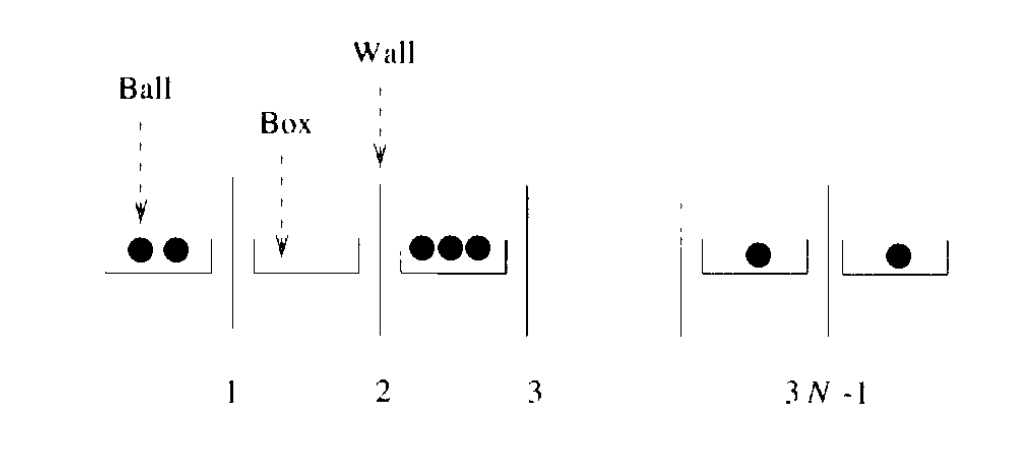
\includegraphics[width=0.5\linewidth]{image.png}
         \caption{Regiões de Temperatura Positiva e Negativa para um Sistema de Energia Limitada}
         \label{fig:enter-label}
     \end{figure}
Em $U = U^{*}$, a temperatura é positiva para $U < U^{*}$ e negativa para$ U > U^{*}$ (figura 1). Note que as temperaturas $T = +\infty$ e $T = -\infty $ correspondem ao mesmo estado, $T^{-1} = 0$. Além disso, um estado de temperatura negativa tem maior energia e, consequentemente, é mais quente que um estado de temperatura positiva. A declaração de Clausius sobre a segunda lei nos diz que o calor não flui espontaneamente de um corpo mais frio para um corpo mais quente, então o sistema não pode ser aquecido a uma temperatura infinita ou negativa por um influxo de calor, desde que seus arredores estejam a uma temperatura positiva finita. O calor sempre fluirá para fora de um sistema de temperatura negativa em contato com um sistema de temperatura positiva.

No entanto, é possível criar um estado de temperatura negativa por meios indiretos. O exemplo clássico é o de uma coleção de momentos magnéticos de núcleos atômicos, que interagem muito fracamente com os demais graus de liberdade em seu material hospedeiro e podem ser considerados efetivamente como um sistema isolado. A energia de um momento magnético (ou spin, para simplificar) é apenas aquela devido à sua orientação em um campo magnético aplicado. O sistema tem sua energia mínima quando todos os spins estão paralelos ao campo e sua energia máxima quando todos estão antiparalelos ao campo. O estado de temperatura infinita de entropia máxima corresponde a orientações completamente aleatórias dos spins. Em uma temperatura positiva baixa, os spins estarão predominantemente paralelos ao campo. Se a direção do campo for invertida rapidamente, os spins se encontrarão predominantemente antiparalelos ao campo e, portanto, em um estado de temperatura negativa.
     
     \item \textbf{Problema 2.3} Compare a diminuição na entropia do cérebro de um leitor durante a leitura de um livro com o aumento na entropia devido à iluminação (por meio de uma lâmpada elétrica).
 \end{itemize}
\textbf{Resposta:} A alteração na entropia resultante da assimilação de uma quantidade $\Delta I$ de informações (medida em bits) é "atribuída a \textbf{Claude Shannon}, o pai da teoria da informação, ele introduziu essa relação em seu artigo seminal de 1948, "A Mathematical Theory of Communication"
\[
\Delta S = -\frac{k}{\log_{2} e} \Delta I
\]
"A equação descreve a relação entre a mudança na entropia de um sistema e a quantidade de informações que ele assimila. O sinal negativo indica que a obtenção de informações leva a uma diminuição da entropia, o que se alinha à ideia de que as informações representam ordem e reduzem a incerteza."
Um livro que usa apenas o alfabeto latino e os sinais de pontuação requer cerca de $2^5
$ caracteres diferentes, portanto, são necessários 5 bits para especificar qualquer caractere. Assim, o conteúdo de informações de um livro de 400 páginas, em que cada página tem 50 linhas de 70 caracteres cada, é de$\Delta I=5×70×50×400=7×10^6$ bits. Então $\Delta S_ \text{brain}∼−10^{−16}  \text{J K}^{−1}$. Por outro lado, uma lâmpada elétrica que emite uma potência $P$ de, digamos, $100 W$ em seu entorno a uma temperatura $ T=300 K$ causa um aumento de entropia 
\[
\Delta S_{\text{bulb}} \sim \frac{Pt}{T} \sim 0.3t \text{ J K}^{-1}
\]
em que $t$ é o tempo (em segundos) gasto pelo processo de leitura. Temos então
\[
\frac{\Delta S_{brain}}{\Delta S_{bulb}} \sim - \frac{10^{-19}}{t^*}
\]
onde $t^*$ é o tempo medido em horas. Para tempos típicos de leitura (digamos, algumas horas), essa proporção é minúscula. Claro, ela será ainda menor se levarmos em conta a produção de entropia por todos os processos metabólicos do corpo do leitor, bem como a da lâmpada. 

\textbf{Problema 2.11} Aproximadamente $10^{-4}$ segundos após o Big Bang, o conteúdo material do Universo primordial consistia principalmente em elétrons e pósitrons $e^{\pm }$, neutrinos $\nu$ e fótons $\gamma$, todos em equilíbrio térmico a uma temperatura de cerca de $10^{12}$ K. O volume $V$ de uma região 'co-móvel' do espaço se expande com o tempo e, enquanto o número de partículas em um gás relativístico ocupando essa região for constante, a temperatura desse gás cai, com $T^3 \propto V^{-1}$. À medida que a temperatura caiu para cerca de $10^{11}$ K, a taxa de interações entre os neutrinos e as outras partículas tornou-se desprezível e, a partir de então, a evolução do gás de neutrinos estava completamente desacoplado daquele dos elétrons, pósitrons e fótons. A uma temperatura de cerca de $6 x 10^{9}$ K (para a qual $kT$ é igual à energia de repouso de um elétron), elétrons e pósitrons (dos quais havia aproximadamente números iguais) aniquilaram-se rapidamente, produzindo fótons. Como resultado, o gás de fótons restante estava a uma temperatura $T_\gamma$ um pouco mais alta do que a temperatura $T_\nu$ dos neutrinos.

Hoje, a temperatura dos fótons (a radiação cósmica de fundo em micro-ondas) é de cerca de 2,7 K. Encontre a temperatura atual dos neutrinos relíquia, assumindo que o processo de aniquilação foi reversível e que o Universo naquele tempo era espacialmente homogêneo. As densidades de energia dos gases relativísticos em questão são dadas por $u_\nu = cT^4$, $u_e = 2cT^4$ e $u_\gamma = \frac{8}{7}cT^4$, onde c é uma constante. (O fator 2 é responsável pela presença de elétrons e pósitrons e o fator de $\frac{8}{7}$ pela diferença entre as estatísticas de Bose e Fermi.)

\textbf{Resposta:} Um instante antes da aniquilação de $e^{\pm }$, neutrinos e fótons estavam na mesma temperatura, digamos, $T$. Consideramos uma região do espaço cujo volume naquele momento era $V$. Um curto tempo depois, quando a aniquilação estava completa, o volume havia aumentado, digamos, para $V'$. Chamamos a temperatura do fóton neste momento posterior de $T'_\gamma$ e a temperatura do neutrino de $T'_\nu$. Desde então, ambas as temperaturas caíram pelo mesmo fator, então sua razão agora é
\[
\frac{T^\text{agora}_\nu}{T^\text{agora}_\gamma}=\frac{T'_\nu}{T'_\gamma}
\]
 e precisamos calcular essa razão.
 Os neutrinos não foram afetados pela aniquilação, então temos
\[
V T^3 = V' T'^3_\nu
\]

Se o Universo fosse homogêneo, não haveria gradiente de temperatura e, portanto, nenhum fluxo de calor. Consequentemente, se o processo de aniquilação fosse reversível (o que é uma questão de suposição), então a entropia total da região considerada permaneceria constante. Será, portanto, útil encontrar as entropias dos gases em termos de seu volume e temperatura. A partir da primeira lei, a energia total $U$ e a entropia $S$ de um gás em um volume $V$ estão relacionadas por 
\[
\left( \frac{\partial U}{\partial T} \right)_V = T \left( \frac{\partial S}{\partial T} \right)_V
\]
 e, se $U = cT^4V$, podemos integrar essa relação para obter $ S = \frac{4}{3}cT^3V$. Nosso resultado anterior mostra que a entropia dos neutrinos permanece inalterada, e agora podemos descobrir o que está implícito na suposição de que a entropia do gás elétron-fóton também permanece inalterada. Imediatamente antes da aniquilação, a entropia no volume $V$ era
\[
S = S_e + S_\gamma = \frac{4}{3} \times 2cT^3V + \frac{4}{3} \times \frac{8}{7} cT^3V = \frac{88}{21} cT^3V
\]
 Após a aniquilação, a entropia dos fótons a uma temperatura $T'_\gamma$', em um volume $V'$, era 
 \[
 S' = \frac{4}{3} \times \frac{8}{7} c T_y'^3 V' = \frac{32}{21} c T_y'^3 V'
 \]
 Igualando S e S' e, em seguida, usando nosso primeiro resultado, descobrimos que 
 \[
 T_y'^3 = \frac{11}{4} \frac{V}{V'} T^3 = \frac{11}{4} T_v'^3
 \]
Como a razão dos volumes $\frac{V}{V'}$ se cancela, não importa exatamente quais dois instantes de tempo escolhemos antes e depois da aniquilação. Na verdade, poderíamos ter assumido que a aniquilação foi instantânea (e assim $V' = V$) e obtido o mesmo resultado, mas essa suposição não é totalmente realista. Assim, a razão $\frac{T'_\nu}{T'_\gamma}$' é igual a $\left( \frac{4}{11} \right)^{1/3}$ e a temperatura atual do neutrino é 
\[
T_v^\text{now} = \left( \frac{4}{11} \right)^{1/3} \times 2.7 \text{ K} \simeq 1.9 \text{ K}
\]


\end{document}
